\section{Monitoring and Calibration Suites}
\label{sec:calibration}

\subsection{Framework}

A calibration framework was developed to implement visualization software tools needed for all detector
systems. Standard views were developed using the Java {\it Swing} application to visualize detector components
and to provide call-back mechanisms necessary to display detector-component specific information.  These
software tools provide functionality for data fitting, plotting, and displaying using a Graphical User Interface
(GUI) environment.

The calibration framework makes use of the other CLAS12 libraries (the geometry and plotting packages, as well
as database utilities) and provides a uniform GUI for all calibration applications. The framework provides a
data-processing interface and a calibration constant database interface used for online and offline data analysis.

A common data-streaming interface is implemented with software-level abstraction that allows the calibration and
monitoring codes to run on all of the supported data formats used in CLAS12, including data read in real-time from
the CLAS12 DAQ system~\cite{daq-nim}.

\subsection{Calibration and Monitoring Suites}

The software programs used for the CLAS12 detector subsystem monitoring, as well as the energy and time
calibrations,  are Java-based suites that employ the framework discussed in Section~\ref{common-tools}. The
software tools provided by the framework facilitate the development of detector-specific suites.
Figure~\ref{suites} shows representative views of the CLAS12 subsystem calibration suites.

\begin{figure*}
\centering
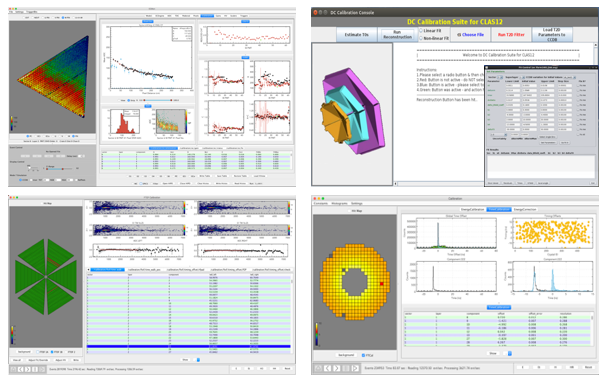
\includegraphics[width=2.0\columnwidth]{pics/suites.png}
\caption{Representative subsystem calibration GUIs for the Electromagnetic Calorimeter (ECAL)~\cite{ecal-nim}
  (upper left), Drift Chambers (DC)~\cite{dc-nim} (upper right), Forward Time-of-Flight (FTOF)~\cite{ftof-nim}
  (lower left),  and Forward Tagger (FT)~\cite{ft-nim} (lower right).}
\label{suites}
\end{figure*}

The calibration applications take as input raw or reconstructed data files (from either beam data or Monte Carlo
simulations) in either EVIO or HIPO data formats.  They display and fit the various quantities and histograms
relevant to the extraction of the calibration constants.  The calibration analysis parameters are saved into ASCII
files with the same structure as the tables defined in CCDB.  The constants are then reviewed and uploaded to the
database using CCDB commands.

\section{CLAS12 Event Display}
\label{sec:ced}

The CLAS12 Event Display ({\it ced}) is a diagnostic graphical application for displaying CLAS12 events. The
primary element of {\it ced} is the ``view'', i.e. a graphical representation of CLAS12 in its entirety or a subset of
its detector subsystems. For a given event, the primary purpose is to display the detector components that have
recorded a signal, and, if available, the reconstructed tracks, to provide a visualization of the particle passage
through the detector. In addition, {\it ced} can display information about the event such as the data banks, or
information about the detector, such as the magnetic fields. Available views are both 2- and 3-dimensional with
the possibility of disabling the latter for faster execution.

An illustration of views in {\it ced} is shown in Fig.~\ref{fig:dcTracks}, where a section of CLAS12 is displayed in
a cut-view with a specific focus on the Forward Detector. The colored areas in the space around the detectors
indicate regions where a significant magnetic field intensity is present from either the solenoid or torus;
reconstructed tracks are shown by the orange lines. Similarly, Fig.~\ref{fig:ced} shows views of the Central
Detector and of the Forward Tagger. Figure~\ref{fig:ced}(left) shows two tracks originating from the target as
reconstructed from the fit of the available central tracker hits in correlation with signals in the outer detectors.
Here, the color scale is representative of the recorded signal intensity. Figure~\ref{fig:ced}(right) shows a
front view of the Forward Tagger calorimeter for an event where three clusters were recorded. {\it ced} is
designed to be operated offline, reading either raw EVIO or HIPO events from a file, or online, reading events
from the CLAS12 DAQ system~\cite{daq-nim} to allow for real-time monitoring of the detector during data taking.

\begin{figure*}
\centering
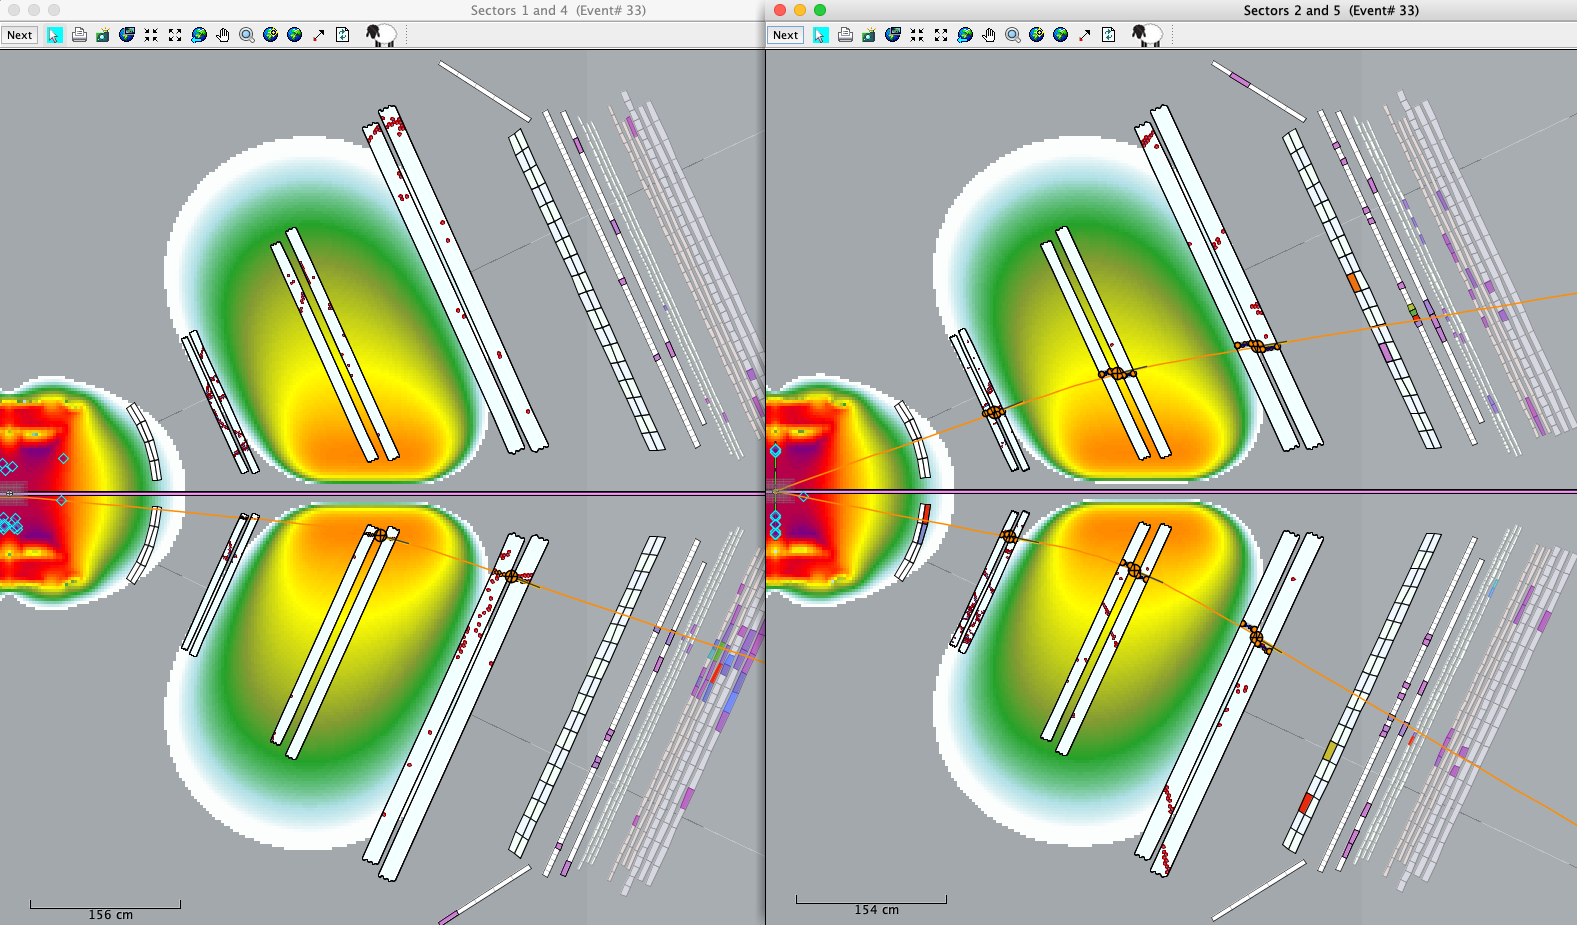
\includegraphics[width=0.95\textwidth]{pics/dcTrack3.png}
\caption{Views from {\it ced} of charged particle tracks in the DC showing cut-views to highlight different pairs
  of sectors of the CLAS12 Forward Detector. The colored detector elements are the registered hits and the
  orange lines are the result of track reconstruction using the hits in the DCs. The colored areas about the
  detectors represent the regions of magnetic field from the torus and the solenoid. In these views the beam is
  incident from the left and the target is located in the middle of the solenoid (at the left edge of the image).}
\label{fig:dcTracks}
\end{figure*}

\begin{figure*}
\centering
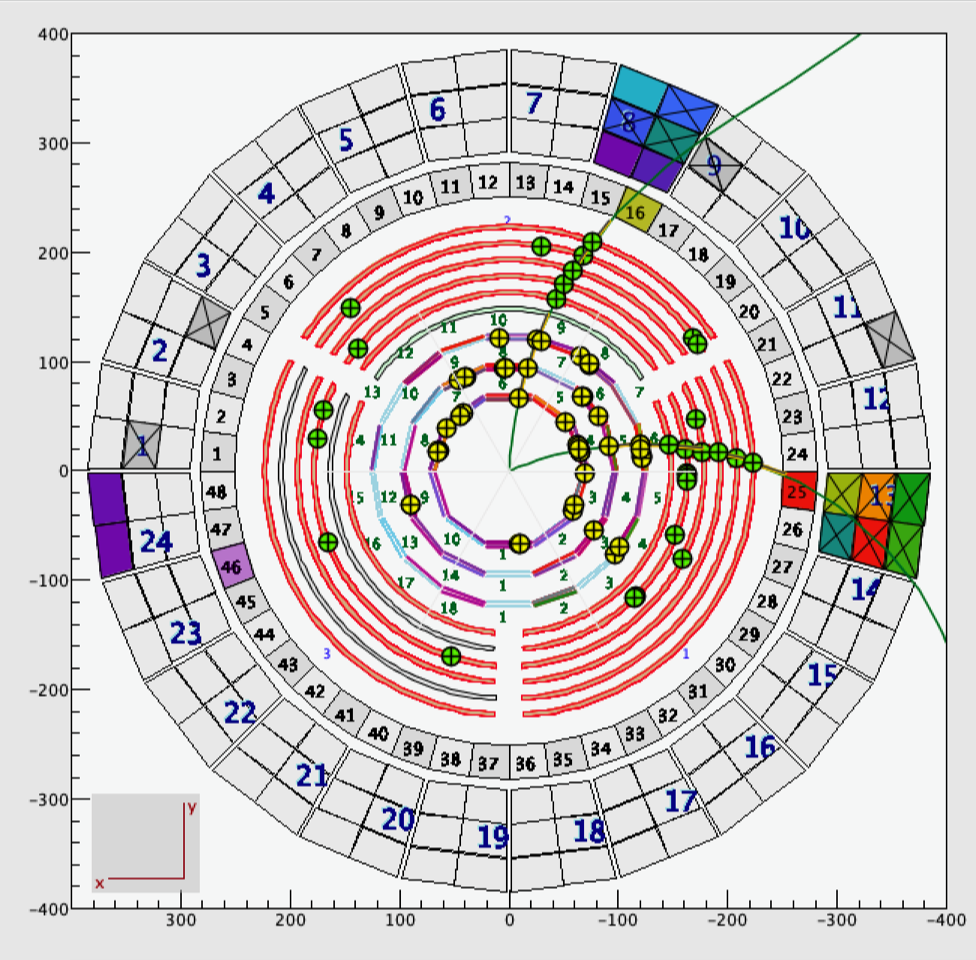
\includegraphics[width=0.4\textwidth]{pics/ced_central.png}
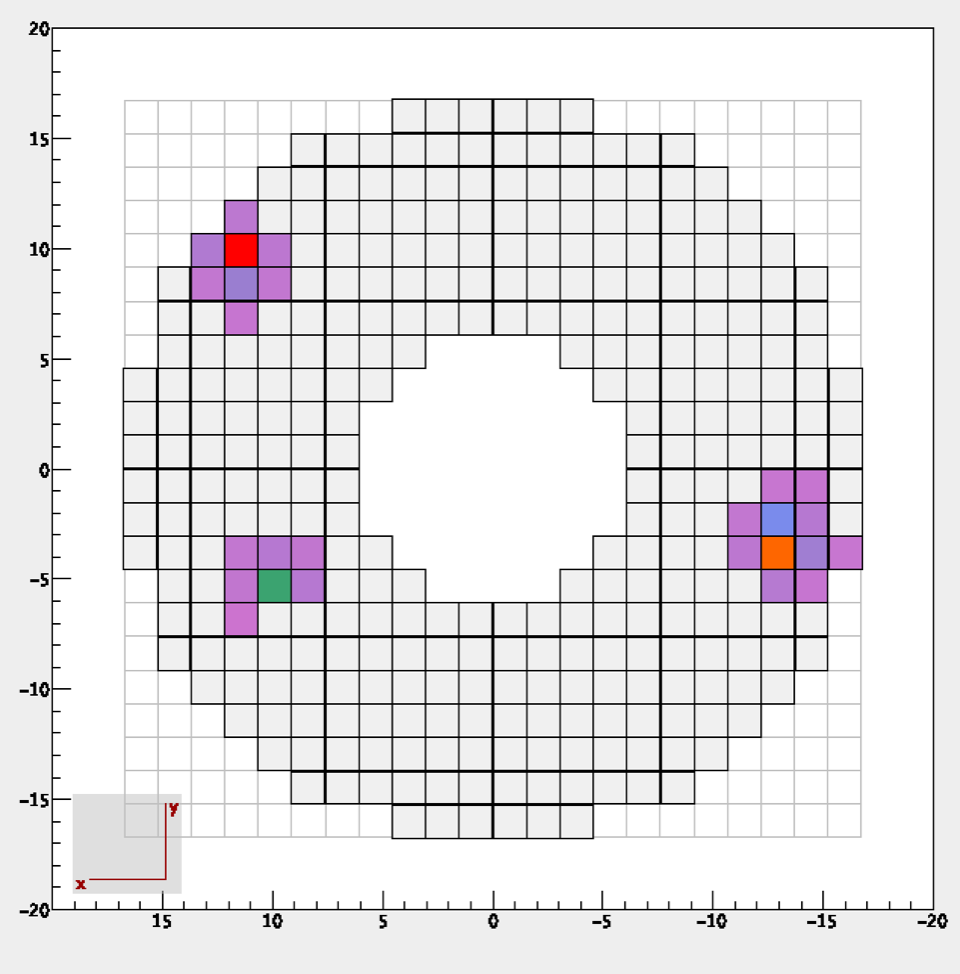
\includegraphics[width=0.39\textwidth]{pics/ced_ft.png}
\caption{Views from {\it ced} of the Central Detector (left) and the Forward Tagger (right) from a view looking
  down the beamline. In the Central Detector view (left), two tracks originating from the target are shown as
  reconstructed from the fit of the available central tracker hits in correlation with signals in the outer detectors
  (Central Time-of-Flight (CTOF) and Central Neutron Detector (CND)). Here the color scale is representative of
  the recorded signal intensity. The right figure shows a front view of the Forward Tagger calorimeter for an event
  where three clusters were recorded.}
\label{fig:ced}
\end{figure*}
